\documentclass[tikz,border=5pt]{standalone}
\usepackage{pgfplots}
\usepgfplotslibrary{groupplots}
\pgfplotsset{compat=1.18}

\definecolor{corba}{HTML}{365FB3}
\definecolor{esquerra}{HTML}{D97706}
\definecolor{dreta}{HTML}{15803D}

\begin{document}
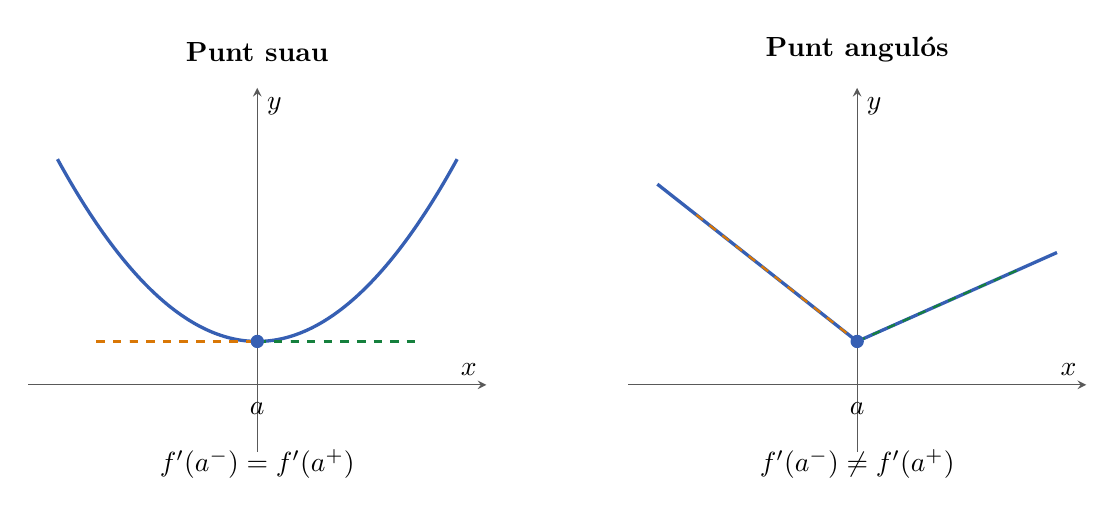
\begin{tikzpicture}
  \begin{groupplot}[
    group style={group size=2 by 1, horizontal sep=1.8cm},
    width=7.4cm,
    height=6.2cm,
    axis lines=middle,
    xmin=-2.35,
    xmax=2.35,
    ymin=-1,
    ymax=4.45,
    xlabel={$x$},
    ylabel={$y$},
    xtick=\empty,
    ytick=\empty,
    axis line style={black!65},
    tick style={black!65},
    clip=false,
  ]
    % Punt suau: les dues derivades laterals coincideixen.
    \nextgroupplot[title={\textbf{Punt suau}}]
      \addplot[corba, very thick, domain=-2.05:2.05, samples=150]
        {0.65*x^2+0.65};
      \addplot[only marks, mark=*, mark size=2.2pt, corba]
        coordinates {(0,0.65)};
      \addplot[esquerra, dashed, thick, domain=-1.65:0] {0.65};
      \addplot[dreta, dashed, thick, domain=0:1.65] {0.65};
      \node[anchor=north] at (axis cs:0,-0.12) {$a$};
      \node[anchor=north] at (axis cs:0,-0.82)
        {$f'(a^-)=f'(a^+)$};

    % Punt angulós: les dues pendents laterals són diferents.
    \nextgroupplot[title={\textbf{Punt angulós}}]
      \addplot[corba, very thick, domain=-2.05:0, samples=80]
        {-1.15*x+0.65};
      \addplot[corba, very thick, domain=0:2.05, samples=80]
        {0.65*x+0.65};
      \addplot[only marks, mark=*, mark size=2.2pt, corba]
        coordinates {(0,0.65)};
      \addplot[esquerra, dashed, thick, domain=-1.65:0]
        {-1.15*x+0.65};
      \addplot[dreta, dashed, thick, domain=0:1.65]
        {0.65*x+0.65};
      \node[anchor=north] at (axis cs:0,-0.12) {$a$};
      \node[anchor=north] at (axis cs:0,-0.82)
        {$f'(a^-)\ne f'(a^+)$};
  \end{groupplot}
\end{tikzpicture}
\end{document}

